\pagecolor{gray!10}
Full Name: \hfill AP Calculus BC \\[22pt]
Date: \hfill Chapter 1 Practice Test \\[22pt]
\textbf{Multiple Choice Section} \hfill \textbf{20 Minutes; No Calculator} \\[11pt]

\begin{center}
    \textbf{Show All Work}
\end{center}
\vspace{11pt}

\begin{questions}
    %Question 1
    \question Which of the following equations is true? \\

    \begin{oneparchoices}
        \choice $\diff \left[\cot^{-1} (4x)\right] = -\dfrac{4}{16x^2 + 1}$
        \choice $\diff \left[e^{\cos (x)}\right] = -e^{-\sin (x)}\cos (x)$ \vspace{11pt}
        \choice $\diff \left[\ln^3 \left(1 - x^2\right)\right] = \dfrac{3\ln^2 \left(1 - x^2\right)}{1 - x^2}$ 
        \choice $\diff \left[e^{2x}\cos^{-1} (x)\right] = \dfrac{2e^{2x}}{\sqrt{1 - xe^2}}$
    \end{oneparchoices} \par \horizontalline

    %Question 2
    \question If $f(x) = \cot^{-1} (\sin (x))$, then $\diff [f(x)] = $ \\

    \begin{oneparchoices}
        \choice $-\csc^2 (\sin (x)) \cos^2 (x)$
        \choice $\sec (x)$
        \choice $\dfrac{\cos (x)}{1 + \sin^2 (x)}$
        \choice $-\dfrac{\cos (x)}{1 + \sin^2 (x)}$
        \choice $-1$
    \end{oneparchoices} \par \horizontalline

    %Question 3
    \question Let $y = f(x)$ be a solution to the differential equation $\deriv = x - y^2 \forcespace$ with the initial condition $f(0) = 1$. What is the best approximation for $f(2)$ if Euler's Method is used, starting at $x = 0$ with a step size of $1.0$ \\
    
    \begin{oneparchoices}
        \choice $-1$
        \choice $0$
        \choice $1$
        \choice $2$
        \choice $3$
    \end{oneparchoices} \par \horizontalline

    \newpage

    %Question 4
    \question Selected values of $f$, $g$, and their derivatives are indicated in the table below. Let $h(x) = g\left(f\left(\sqrt{x}\right)\right)$. What is the value of $h'(4)$? \begin{align*}
        \arraycolsep=22pt\def\arraystretch{1.5} 
        \begin{array}{|c|c|c|c|c|}
            \hline
            x & f(x) & g(x) & f'(x) & g'(x) \\ \hline
            2 & 4 & 3 & 4 & -1 \\ \hline
            4 & 2 & -1 & 7 & 8 \\ \hline
            16 & 1 & 2 & 2 & 1 \\
            \hline
        \end{array}
    \end{align*}

    \begin{oneparchoices}
        \choice $6$
        \choice $\dfrac{1}{4}$
        \choice $1$
        \choice $2$
        \choice $24$
    \end{oneparchoices} \par \horizontalline

    %Question 5
    \question The figure below shows the graph of the functions $f$ and $g$. If $B(x) = \dfrac{g(x)}{f(x)}$. what is $B'(6)$?
    \begin{center}
        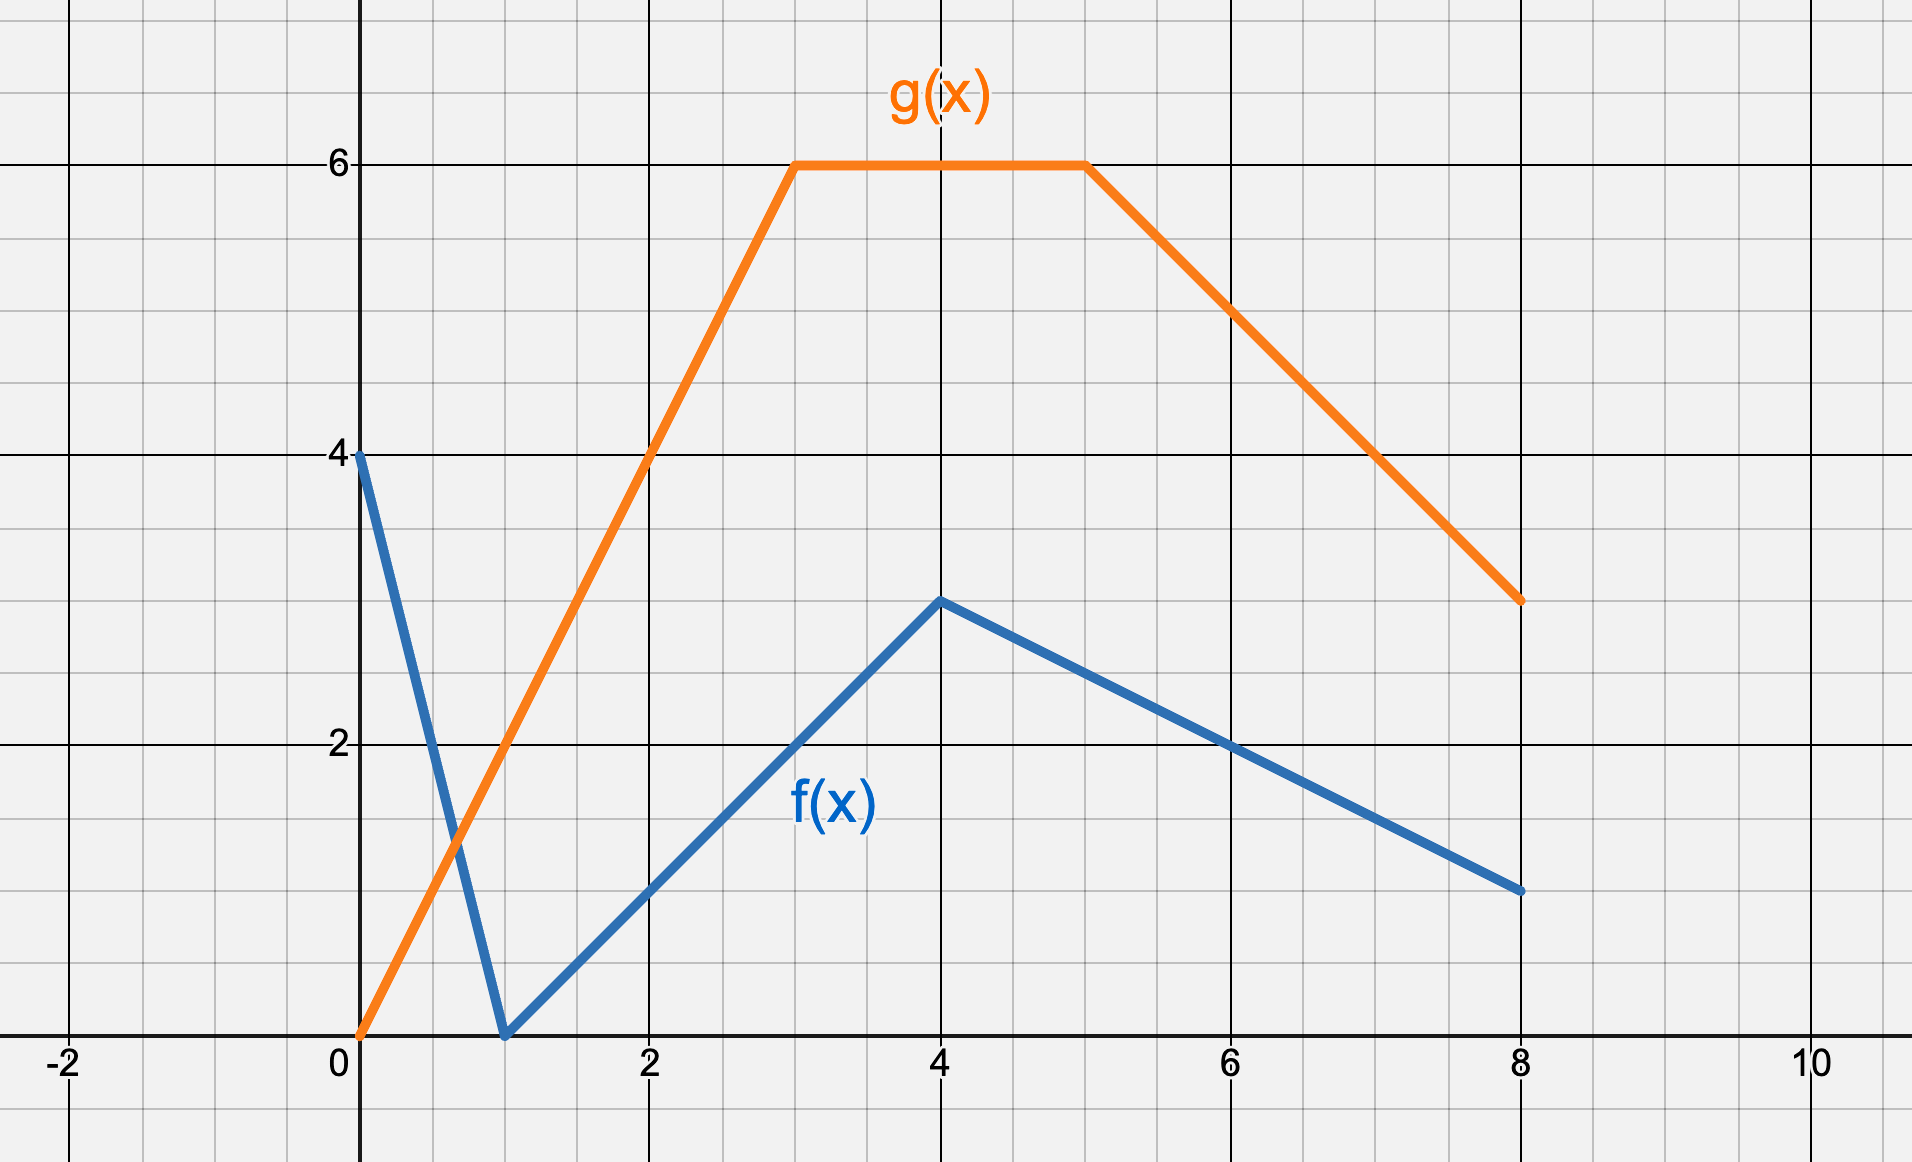
\includegraphics[width = 0.6\textwidth]{\graphicsdir Chapter 1 Graphics/PT-Graphic1.png}
    \end{center} \vspace{11pt}

    \begin{oneparchoices}
        \choice $-\dfrac{9}{2}$
        \choice $\dfrac{1}{8}$
        \choice $-2$
        \choice $0$
        \choice $DNE$
    \end{oneparchoices} \par \horizontalline

    %Question 6
    \question If $f(x) = 3\sin (x) + 4\cos^2 (x)$, then $f''\left(\dfrac{\pi}{2}\right)$ \\

    \begin{oneparchoices}
        \choice $3$
        \choice $0$
        \choice $5$
        \choice $-8$
        \choice $-3$
    \end{oneparchoices} \par \horizontalline

    \newpage

    %Question 7
    \question Which of the following is an equation of the line tangent to the graph of $f(x) = x^6 + x^5 + x^2$ at the point where $f'(x) = -1$? \\

    \begin{oneparchoices}
        \choice $-3x - 2$
        \choice $-3x + 4$
        \choice $-x + 0.905$ \\[11pt]
        \makebox[0.23 \textwidth] \choice $-x + 0.271$
        \makebox[0.27 \textwidth]\choice $-x - 0.271$
    \end{oneparchoices} \par \horizontalline

    %Question 8
    \question A biologist is tracking the growth of a circular colony of bacteria in a Petri dish. She observes that the colony is expanding at rate of $15 \si{mm^2 \per hour}$. Find the rate at which the radius is increasing when the diameter is $5 \si{mm}$. \\

    \begin{oneparchoices}
        \choice $3$
        \choice $3\pi$
        \choice $\dfrac{3}{\pi}$
        \choice $\dfrac{3}{2\pi}$
        \choice $\dfrac{3\pi}{2}$
    \end{oneparchoices} \par \horizontalline

    %Question 9
    \question What is the slope of the line tangent to the curve $y^2 + x = -2xy - 5$ at the point $(2, 1)$? \\

    \begin{oneparchoices}
        \choice $-\dfrac{4}{3}$
        \choice $-\dfrac{3}{4}$
        \choice $-\dfrac{1}{2}$
        \choice $-\dfrac{1}{4}$
        \choice $0$
    \end{oneparchoices} \par \horizontalline
\end{questions}

\newpage
\stepcounter{sectioncount}

\textbf{Free Response Section} \hfill \textbf{45 Minutes; No Calculator} \\[11pt]

\begin{center}
    \textbf{Show All Work}
\end{center}
\vspace{11pt}

\begin{questions}
    \question Compute the following derivatives. \\

    \begin{parts}
        \part $\diff \left[\sin^{-1} \left(e^{2x}\right)\right]$

        \vfill

        \parthline

        \part $\diff \left[\ln \left(\cot \left(\sqrt{x}\right)\right)\right]$

        \vfill
    \end{parts} \horizontalline

    \newpage

    \question Let $f(x)$ be the function defined by $f(x) = \sin \left(\dfrac{\pi}{2}\right)x$, let $g(x)$ be a differentiable function with selected values for $g(x)$ and $g'(x)$ given in the table below, and let $h(x)$ be a differentiable function whose graph is given below. \\
    \begin{minipage}[t]{0.75\textwidth} \vspace{0pt}%
        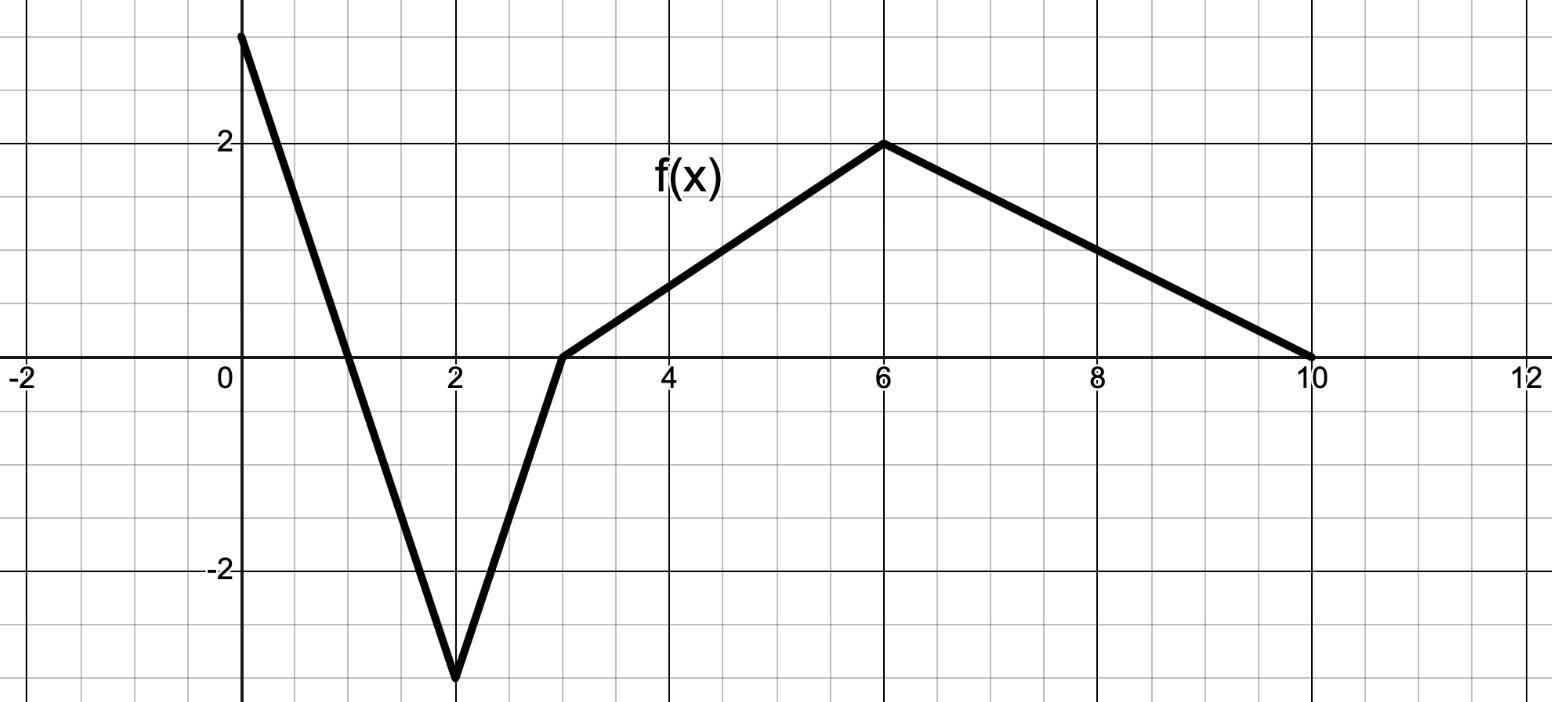
\includegraphics[width = 0.9\textwidth]{\graphicsdir Chapter 1 Graphics/PT-Graphic2.png}
    \end{minipage} \hfill \begin{minipage}[t]{0.2\textwidth} \vspace{11pt}% 
        \def\arraystretch{1.4}
        $\begin{array}{|c|c|c|}
            \hline
            x & g(x) & g'(x) \\ \hline
            0 & -2 & 12 \\ \hline
            2 & 0 & -3 \\ \hline
            4 & 5 & 5 \\ \hline
            6 & 3 & 8\\ \hline
            8 & -4 & 11 \\
            \hline
        \end{array}$
    \end{minipage} \\[11pt] \horizontalline

    \begin{parts}
        \part Find the equation of the line tangent to $h(x)$ at $x = 8$.

        \vfill
        
        \parthline

        \part Let $K$ be the function defined by $K(x) = g(f(x))$. Find $K'(6)$.

        \vfill

        \parthline

        \newpage

        \part Let $M$ be the function defined by $M(x) = g(x) \cdot f(x)$. Find $M'(4)$.

        \vfill

        \parthline

        \part Let $J$ be the function defined by $J(x) = \dfrac{h(x)}{g\left(\dfrac{1}{2}x\right)}$. Find $J'(8)$.

        \vfill
    \end{parts} \horizontalline

    \newpage

    \question If $F(x) = \ln \left(3x^2 - 2x + 1\right)$, find $F''(x)$. 

    \vfill
    
    \horizontalline

    \question Find the equations of the lines tangent and normal to $g(x) = e^{4x}\cos (x)$ at $x = 0$ and use it to approximate $g(-0.2)$

    \vfill

    \horizontalline

    \newpage

    \question Consider the curve given by $2y - x + xy = 8$ 

    \horizontalline

    \begin{parts}
        \part Show that $\deriv = \dfrac{1 - y}{2 + x}$.

        \vfill

        \parthline

        \part Find the coordinates of the point(s) where the tangent line is horizontal or prove why there is no such point(s). 

        \vfill

        \parthline

        \newpage

        \part Find the value of $\deriv[2] \forcespace$ at $(1, 3)$. Does the curve have a relative maximum, a relative minimum, or neither at $(0, 1)$? Justify your answer.

        \vfill
    \end{parts} \horizontalline

    \newpage

    \question Two people on bikes are at the same place. One of the bikers starts riding directly north at a rate of $8 \si{m \per sec}$. Five seconds after the first biker started riding north, the second starts to ride directly east at a rate of $5 \si{m \per sec}$ At what rate is the distance between the two riders increasing $20$ seconds after the \textit{second} person started riding? 

    \vfill

    \parthline
\end{questions}

\newpage

\pagecolor{white}